% Parallelschwingkreis R||L||C - Impedanzbetrag |Z|
% Halblogarithmische Darstellung für Symmetrie um w0
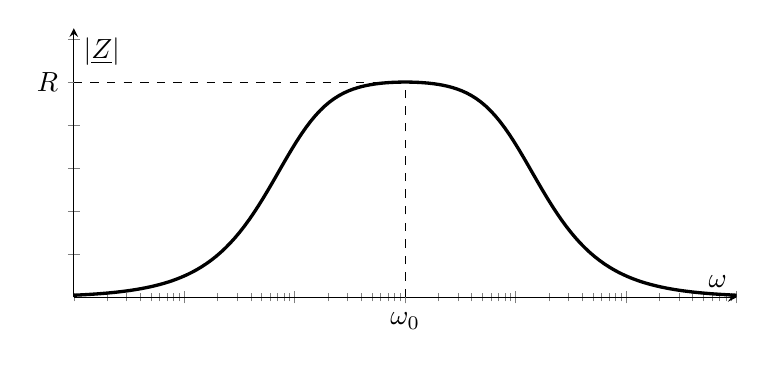
\begin{tikzpicture}[x=1cm,y=1cm]
    \begin{axis}[
        % xaxis log, yaxis linear
        xmode=log, ymode=linear,
        xmin=1e0, xmax=1e6,
        domain=1e0:1e6,
        ymin=0, ymax=12.5,
        xlabel={$\omega$},
        ylabel={$|\underline{Z}|$},
        axis x line= center,
        axis y line= center,
        %grid=none,
        width=10cm,
        height=5cm,
        %axis line style={-latex},
        %tick style={color=black},
        %xtick={\empty}, % keine x-Ticks
        xticklabels={},
        %minor xtick={},
        extra x ticks={1e3},
        extra x tick labels={$\omega_0$},
        %ytick={\empty}, % keine y-Ticks
        ytick distance=2,
        yticklabels={\empty},
        extra y ticks={10},
        extra y tick labels={$R$},
        samples=141,
    ]
        %Impedanzbetrag
        \addplot[very thick, black] {1 / (sqrt(0.01 + (x*1e-5 - 1/(x*1e-1))^2 ))}; % |Z(w)| = 1/sqrt( 1/R^2 + (w*C - 1/(w*L)^2) )
        \addplot[dashed, mark=none, black] coordinates {(1e3, 0) (1e3, 10)}; % w0=1e-2, R = 0.1
        \addplot[dashed, mark=none, black] coordinates {(1e0, 10) (1e3, 10)}; % w0=1e-2, R = 0.1
    \end{axis}
\end{tikzpicture}% 
